%%% Template originaly created by Karol Kozioł (mail@karol-koziol.net) and modified for ShareLaTeX use

\documentclass[11pt]{article}

\usepackage[T1]{fontenc}
\usepackage[utf8]{inputenc}
\usepackage{graphicx}
\usepackage{xcolor}
\usepackage{float}
\usepackage{tgtermes}
\usepackage{natbib}
%\usepackage[subnum]{cases}
\usepackage[super]{nth}
\bibpunct{(}{)}{;}{a}{}{,}
\usepackage{amsmath,amssymb}
\usepackage{enumerate}
\usepackage{multicol}
\usepackage{tikz}
\usepackage[amssymb]{SIunits}
\usepackage{rotating}
\usepackage{enumitem}
\usepackage{geometry}
\geometry{total={8.5in,11in},
left=1in,right=1in,%
bindingoffset=0mm, top=1in,bottom=1in}
\usepackage[super]{nth}
\usepackage[
pdftitle={Homework 1}, 
pdfauthor={Jeremy Gibbs, University of Utah},
colorlinks=true,linkcolor=blue,urlcolor=blue,citecolor=blue,bookmarks=true,
bookmarksopenlevel=2]{hyperref}

\linespread{1.1}
\setlength{\parskip}{1em}
\setlength{\parindent}{0pt}
\newcommand{\linia}{\rule{\linewidth}{0.5pt}}

\makeatletter
\renewcommand{\maketitle}{
\begin{center}
\vspace{2ex}
{\huge \textsc{\@title}}
\vspace{1ex}
\\
\linia\\
ME EN 7960-003 \hfill Homework \#2 Solutions \hfill Due: October \nth{7}
\vspace{4ex}
\end{center}
}
\makeatother
%%%

% custom footers and headers
\usepackage{fancyhdr,lastpage}
\pagestyle{fancy}
\lhead{}
\chead{}
\rhead{}
%\lfoot{Assignment \textnumero{} 5}
\cfoot{}
\rfoot{Page \thepage~/~\pageref*{LastPage}}
\renewcommand{\headrulewidth}{0pt}
\renewcommand{\footrulewidth}{0pt}
%

%%%----------%%%----------%%%----------%%%----------%%%

\begin{document}

\title{Large-Eddy Simulation of Turbulent Flows}

\maketitle

%-- Question 1 --%
\vspace{-20pt}
\paragraph{1.) 3D Spectra}~\\\\
Using the isotropic turbulence direct numerical simulation (DNS) data \textit{iso\_vel128.mat} (located on Canvas or at \href{http://gibbs.science/les/homework/iso_vel128.mat}{http://gibbs.science/les/homework/iso\_vel128.mat}) from Lu et al. (2008) calculate the 3D energy spectrum function $E(k)$ where $k = \sqrt{k_1^2 + k_2^2 + k_3^2}$. Make a log-log plot of $E(k)$ vs. $k$. On the plot indicate the isotropic scaling range, the production range, and the dissipation range.
\vspace{50pt}
\begin{figure}[H]
	\centering
	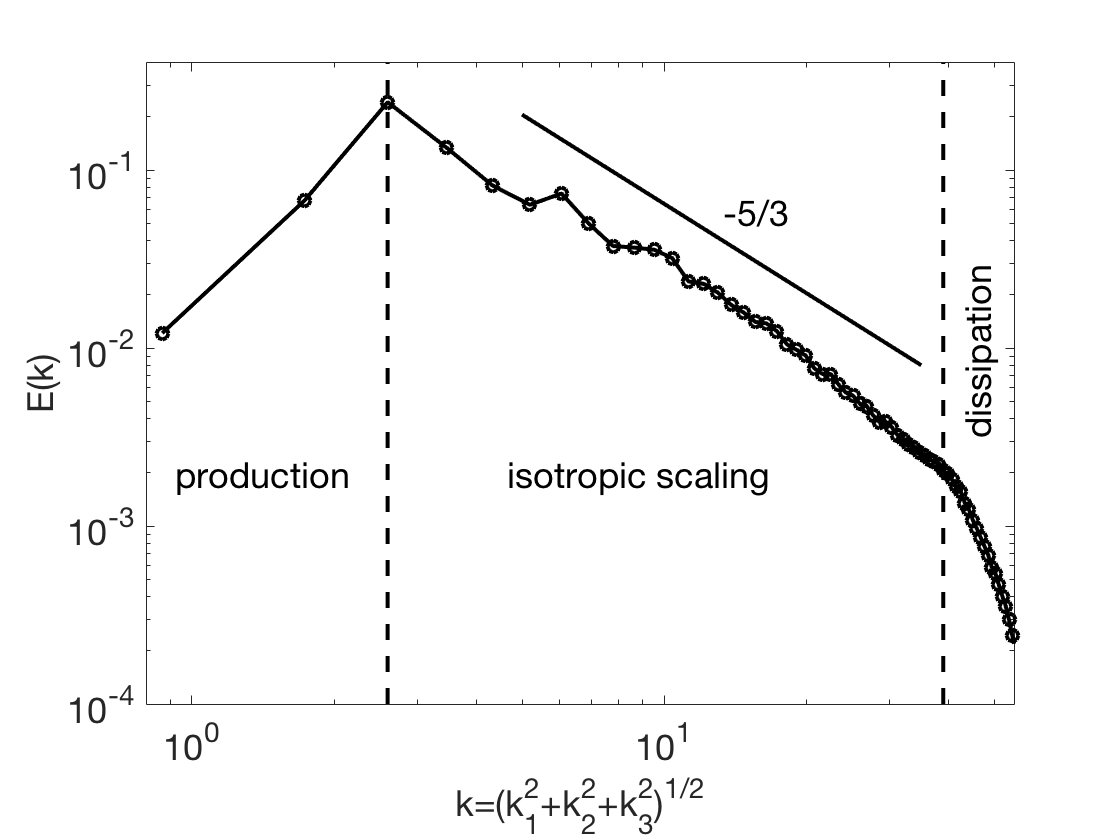
\includegraphics[width=1\textwidth]{3dspectra}
\end{figure}
 
 \textcolor{blue}{Your plot should look similar, although differences might arise depending on your choice of axes limits}
 
%-- Question 2 --%
\paragraph{2.) 3D Filtering: Real Space}~\\\\
Using the data from problem $\#1$ develop a program(s) that applies a 3D filter to the data in real space at two different scales (of your choice) using:
\begin{enumerate}[label=(\alph*),topsep=-10pt]
	\item a 3D spatial box filter
	\begin{figure}[H]
	\centering
	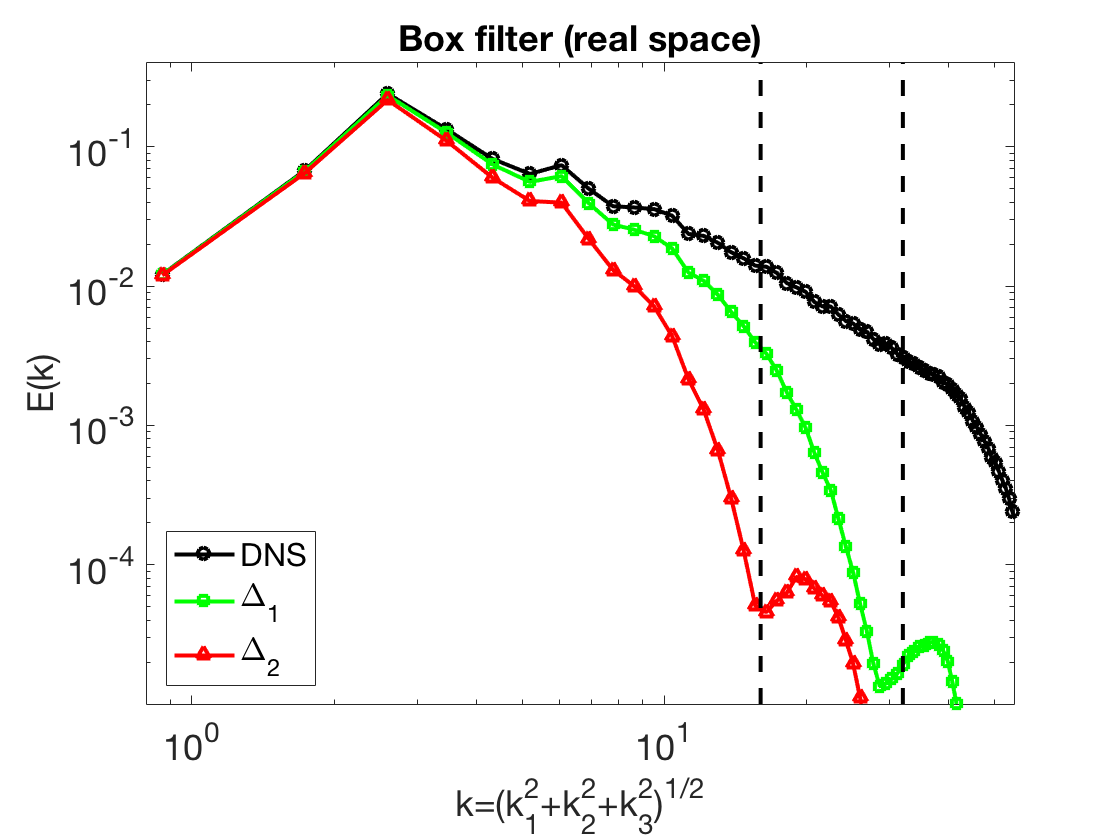
\includegraphics[width=0.63\textwidth]{real_box}
	~\\\textcolor{blue}{Box filter applied in real space at filter widths of $4\Delta$ and $8\Delta$}
	\end{figure}
	\item a 3D Guassian filter
	\begin{figure}[H]
	\centering
	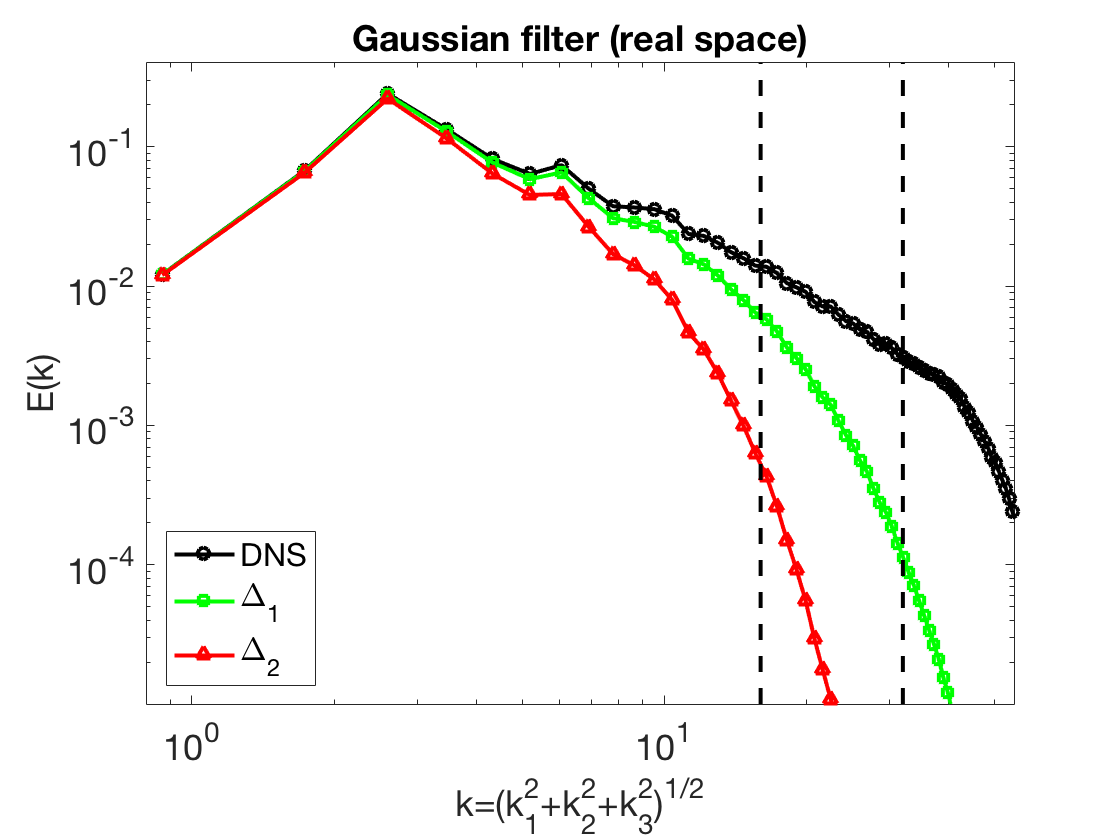
\includegraphics[width=0.65\textwidth]{real_gaussian}
	~\\\textcolor{blue}{Gaussian filter applied in real space at filter widths of $4\Delta$ and $8\Delta$}
	\end{figure}
\end{enumerate}
Present your results by plotting the 3D energy spectrum for each filter type at both filter scales along with the original (unfiltered) energy spectrum from problem \#1. Make a separate plot for each filter type.

%-- Question 3 --%
\paragraph{3.) 3D Filtering: Fourier Space}~\\\\
Using the data from problem \#1 develop a program(s) that applies a 3D filter to the data in Fourier space at two different scales (of your choice) using:
\begin{enumerate}[label=(\alph*),topsep=-10pt]
	\item a spatial box filter
	\begin{figure}[H]
	\centering
	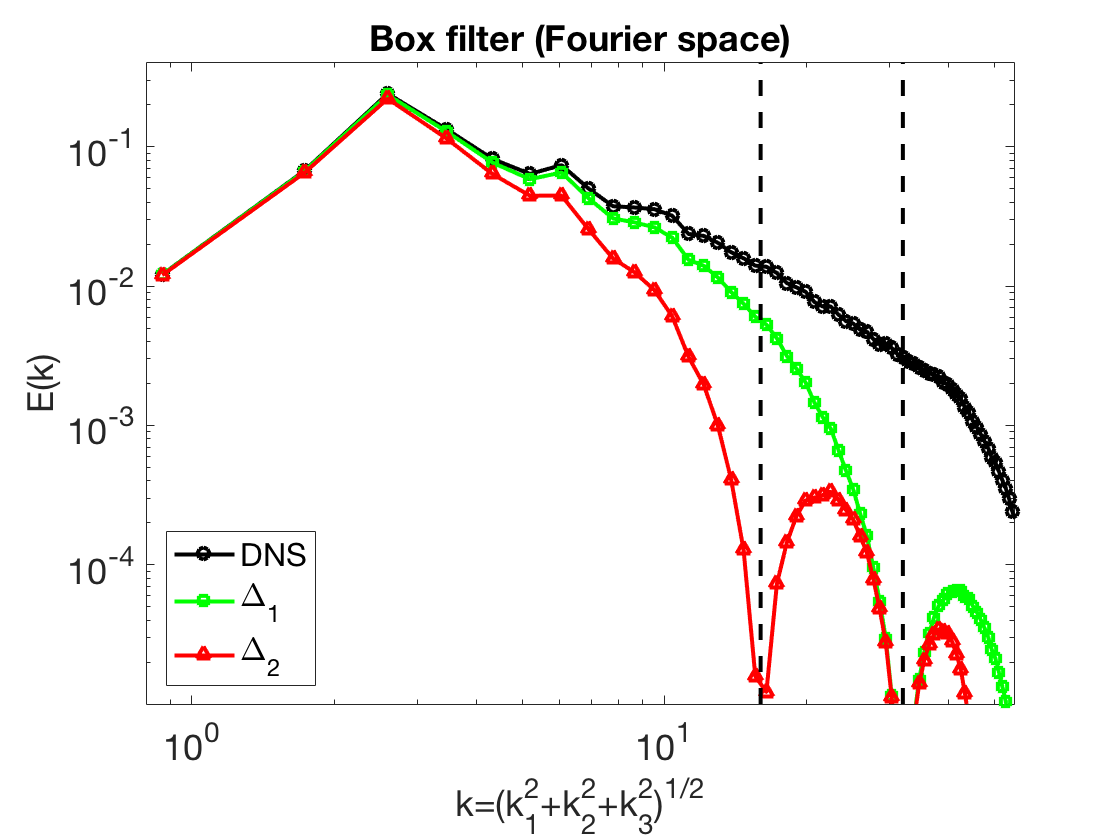
\includegraphics[width=0.65\textwidth]{spectral_box}
	~\\\textcolor{blue}{Box filter applied in Fourier space at filter widths of $4\Delta$ and $8\Delta$}
	\end{figure}
	\item a Guassian filter
	\begin{figure}[H]
	\centering
	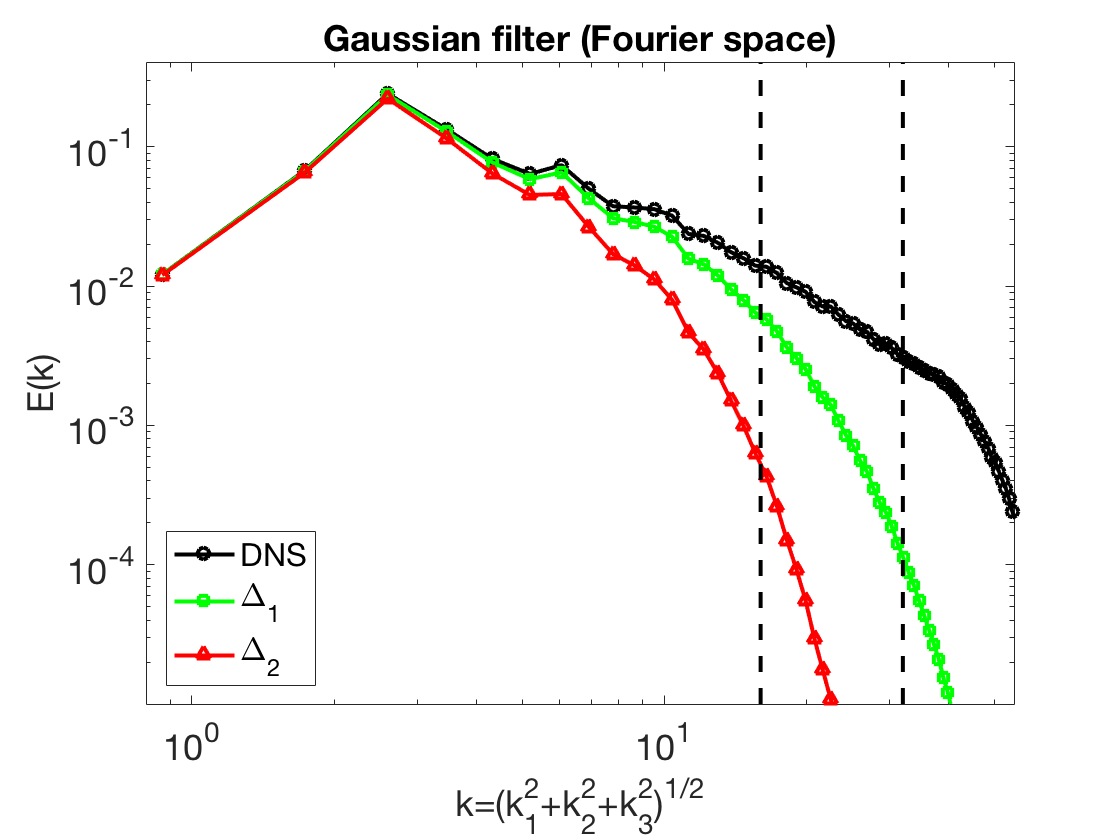
\includegraphics[width=0.65\textwidth]{spectral_gaussian}
	~\\\textcolor{blue}{Gaussian filter applied in Fourier space at filter widths of $4\Delta$ and $8\Delta$}
	\end{figure}
	\vspace{40pt}
	\item a spectral cutoff filter
	\begin{figure}[H]
	\centering
	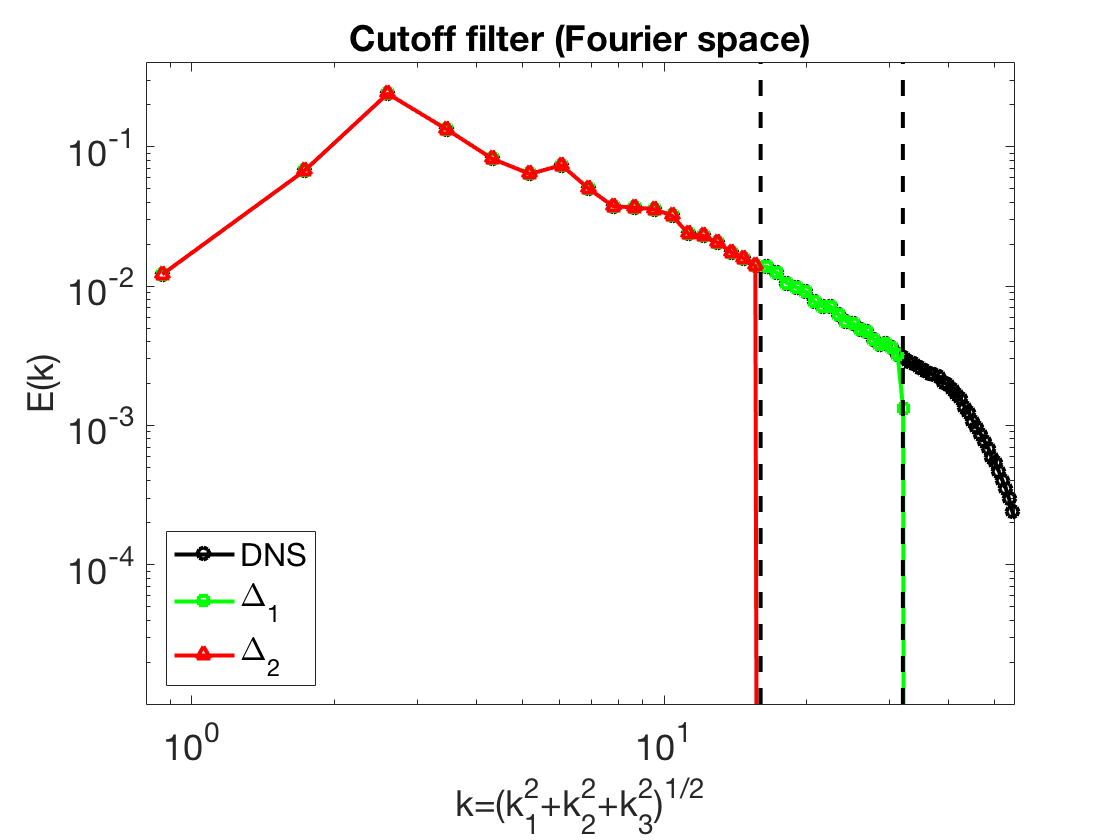
\includegraphics[width=0.65\textwidth]{spectral_cutoff}
	~\\\textcolor{blue}{Cutoff filter applied in Fourier space at $4\Delta$ and $8\Delta$}
	\end{figure}
\end{enumerate}
~\\
Present your results by plotting the 3D energy spectrum for each filter type at both filter scales along with the original (unfiltered) energy spectrum from problem \#1. Make a separate plot for each filter type. For the spatial box filter and the Gaussian filter, compare the execution time for your programs from problems \#2 and \#3.

\textcolor{blue}{Times will vary, but you should have noted that real-space filters are more expensive that Fourier-space filters. In real space, a larger filter is more expensive and the Gaussian filter is more expensive than a box filter.}

\end{document}